\documentclass[11pt]{article}
\input{docs/shared/project_style.tex}
\usepackage{graphicx}
\usepackage{parskip}
\usepackage{tikz}
\usetikzlibrary{arrows.meta,positioning,fit}
\newcolumntype{Y}{>{\RaggedRight\arraybackslash}X}
\definecolor{accent}{HTML}{163A5F}
\definecolor{accent2}{HTML}{EAF3F8}
\definecolor{accent3}{HTML}{F5F7FA}
\newtcolorbox{keybox}{colback=SoftBlue,colframe=TitleBlue,boxrule=0.8pt,arc=2mm,left=3mm,right=3mm,top=2mm,bottom=2mm}
\rhead{Project Plan}

\begin{document}

\DocTitle{Project Plan}{Kinetic MHD-PINN}{Stellarator energetic-particle--Alfvén-eigenmode digital-twin architecture}

\begin{keybox}
\textbf{Purpose.} This document is the single living roadmap for \textbf{Kinetic MHD-PINN}. The top-level \texttt{README.md}, \texttt{project\_plan.tex}, and \texttt{project\_plan.pdf} should be updated whenever the project architecture, interfaces, or module sequence changes.
\end{keybox}

\ProjectTOC

\begin{notebox}
\textbf{Current status.} The repository structure, module boundaries, interface contracts, parallel Python/MATLAB architecture, and a 100-note prerequisite curriculum are established. Thirty basics notes are now substantive standalone textbook drafts, version 1.0, while seventy remain scaffolds. Module 4 now contains the first conventional numerical milestone: a reduced self-adjoint two-harmonic shear-Alfv\'en continuum/eigenmode benchmark with frozen reference outputs, convergence tests, and language-parity criteria. Python execution is verified in the build environment; MATLAB source and tests are complete but have not been executed here. No kinetic drive, orbit-following, transport, or PINN implementation is claimed yet.
\end{notebox}

\section{Project objective}
The project will develop a modular digital-twin framework for energetic particles and Alfv\'en eigenmodes in stellarator burning plasmas. The central scientific objective is to connect magnetic geometry, alpha-particle and neutral-beam distributions, orbit confinement, Alfv\'en eigenmode structure, energetic-particle kinetic drive, fast-ion redistribution, alpha heating, pressure-profile evolution, wall loads, and diagnostics in one controlled multiphysics architecture.

The project is intentionally hierarchical. Early stages use analytic or reduced geometry, low-dimensional mode models, parameterized kinetic closures, and conservative one-dimensional transport. Higher-fidelity interfaces can later accept VMEC-like equilibria, three-dimensional orbit data, external kinetic-MHD calculations, or experimental diagnostic products without changing the top-level module contracts.

\section{Scientific dependency chain}
The nominal causal chain is
\begin{equation}
\begin{aligned}
\text{geometry/equilibrium}
&\rightarrow \text{energetic-particle source}
\rightarrow \text{orbits and losses}
\rightarrow \text{Alfv\'en spectrum}\\
&\rightarrow \text{kinetic drive}
\rightarrow \text{AE transport}
\rightarrow \text{heating and profiles}.
\end{aligned}
\end{equation}
The most important feedback loops are
\begin{equation}
f_f\rightarrow\gamma_{\mathrm{AE}}\rightarrow A_{\mathrm{AE}}\rightarrow D_{\mathrm{AE}}\rightarrow f_f,
\end{equation}
and
\begin{equation}
f_f\rightarrow P_\alpha\rightarrow(T_i,T_e,p,\rho)\rightarrow(v_A,\omega_{\mathrm{AE}},S_\alpha)\rightarrow f_f.
\end{equation}

\section{Educational physics-note architecture}
The repository is also intended to function as a computational-plasma-physics course. In addition to the eleven advanced module notes, \path{docs/physics_notes/basics} contains 100 stable, numbered LaTeX note scaffolds organized into twelve prerequisite parts: mathematical foundations, electromagnetism, elementary plasma physics, MHD, plasma waves, kinetic theory, fusion physics, stellarator foundations, computational methods, multiphysics coupling, physics-informed machine learning, and graph learning.

At this milestone, thirty basics notes have been expanded into substantive standalone textbook drafts, version 1.0. Batch 1 contains Basics 1, 2, 3, 5, 6, 7, 11, 12, 13, and 17. Batch 2 contains Basics 18, 19, 21, 22, 24, 25, 26, 29, 31, and 32. Batch 3 contains Basics 34, 35, 36, 37, 39, 40, 41, 42, 44, and 48, extending the path from ideal-MHD Alfv\'en waves through continuum and gap-mode physics into resonance, phase space, guiding-center dynamics, and energetic-particle distributions. Each draft contains derivations, physical interpretation, computational laboratory guidance, exercises, a symbol table, and references. The remaining seventy notes are still explicitly labeled curriculum scaffolds. Every basics note is maintained as a separate document; the project does not create a combined basics volume. The master course map is compiled as \path{docs/physics_notes/basics/basics_index.pdf}, while \path{docs/physics_notes/basics/curriculum_manifest.json} provides a machine-readable curriculum contract. Advanced module notes progressively add prerequisite tables using stable basics-note numbers and filenames. Module 4 cites Basics 29, 32, 34--37, 69, and 73. Module 5 now cites Basics 32, 34, 35, 37, 39--42, 44, and 48.

\section{Module roadmap}
{\small
\renewcommand{\arraystretch}{1.08}
\begin{longtable}{>{\RaggedRight\arraybackslash}p{0.06\linewidth} >{\RaggedRight\arraybackslash}p{0.30\linewidth} >{\RaggedRight\arraybackslash}p{0.54\linewidth}}
\toprule
\textbf{No.} & \textbf{Module} & \textbf{Purpose}\\
\midrule
1 & Stellarator Equilibrium and Magnetic Geometry & Represent the magnetic configuration, flux surfaces, rotational transform, pressure profile, and equilibrium quantities required by every downstream module.\\
2 & Energetic-Particle Sources and Distribution Functions & Construct alpha-particle and neutral-beam source terms and reduced energetic-particle distributions in energy, pitch, radius, and time.\\
3 & Guiding-Center Orbits, Confinement, and Wall Losses & Follow energetic-particle guiding centers in three-dimensional fields, classify orbits, estimate prompt and delayed losses, and map lost-particle energy to the wall.\\
4 & Alfvén Continuum and Fluid-MHD Eigenmodes & Compute the shear-Alfvén continuum, spectral gaps, mode frequencies, and reduced eigenfunctions before energetic-particle kinetic corrections are added.\\
5 & Kinetic Energetic-Particle Drive and Damping & Evaluate resonant energetic-particle drive and reduced damping contributions to determine whether each Alfvén eigenmode grows or decays.\\
6 & Alfvén-Eigenmode-Induced Fast-Ion Transport & Translate unstable mode amplitudes and resonance structure into energetic-particle redistribution, radial diffusion, convection, and loss enhancement.\\
7 & Alpha Heating and Thermal-Profile Evolution & Convert confined energetic-particle power into electron/ion heating and evolve reduced density, temperature, pressure, and Alfvén-speed profiles.\\
8 & Coupled Kinetic-MHD Multiphysics Integration & Orchestrate the equilibrium, fast-ion, eigenmode, transport, heating, and wall-loss modules with explicit interface contracts and controlled feedback loops.\\
9 & PINN and Neural-Operator Surrogates & Develop and compare PINNs, causal PINNs, neural operators, and structure-preserving surrogates for selected expensive forward and inverse maps.\\
10 & Synthetic Diagnostics and Physics-Informed Inverse Modeling & Generate diagnostic signals from simulated states and reconstruct energetic-particle distributions, mode amplitudes, or profile changes from incomplete observations.\\
11 & GNN Physical Dependency Discovery and Coupling Optimization & Infer directed physical-variable dependencies, feedback groups, state-dependent coupling strengths, and candidate numerical exchange sequences from synthetic interventions.\\
\bottomrule
\end{longtable}
}

\section{Module descriptions and interface anchors}
\subsection{Module 1: Stellarator Equilibrium and Magnetic Geometry}
\textbf{Purpose.} Represent the magnetic configuration, flux surfaces, rotational transform, pressure profile, and equilibrium quantities required by every downstream module.

\textbf{Primary input.} coil or boundary parameters, pressure profile $p(\psi)$, current profile, and equilibrium controls.

\textbf{Primary output.} $\mathbf B(\mathbf x)$, $\psi(\mathbf x)$, $\iota(\psi)$, metric/Jacobian data, and flux-surface geometry.

\textbf{Mathematical anchor.}
\begin{equation}
\nabla p = \mathbf J\times\mathbf B,\qquad \nabla\times\mathbf B=\mu_0\mathbf J,\qquad \nabla\cdot\mathbf B=0.
\end{equation}

\textbf{Surrogate opportunity.} Physics-informed equilibrium surrogate or neural operator over a family of boundary shapes and profiles.


\subsection{Module 2: Energetic-Particle Sources and Distribution Functions}
\textbf{Purpose.} Construct alpha-particle and neutral-beam source terms and reduced energetic-particle distributions in energy, pitch, radius, and time.

\textbf{Primary input.} equilibrium geometry, $n_D$, $n_T$, $T_i$, beam parameters, and source normalization.

\textbf{Primary output.} $S_f(\psi,E,\lambda,t)$, $f_f(\psi,E,\lambda,t)$, birth power, and moments of the fast-ion population.

\textbf{Mathematical anchor.}
\begin{equation}
\frac{\partial f_f}{\partial t}+\dot{\mathbf Z}\cdot\nabla_{\mathbf Z}f_f=C[f_f]+S_f-L_f.
\end{equation}

\textbf{Surrogate opportunity.} Physics-informed or operator-learning surrogate for reduced Fokker--Planck evolution and source-to-distribution maps.


\subsection{Module 3: Guiding-Center Orbits, Confinement, and Wall Losses}
\textbf{Purpose.} Follow energetic-particle guiding centers in three-dimensional fields, classify orbits, estimate prompt and delayed losses, and map lost-particle energy to the wall.

\textbf{Primary input.} $\mathbf B(\mathbf x)$, electric field if retained, particle birth coordinates, energy, pitch, and collision model.

\textbf{Primary output.} orbit histories, confinement fraction, loss time, loss phase space, and $q_{\mathrm{wall}}(\theta,\phi,t)$.

\textbf{Mathematical anchor.}
\begin{equation}
\dot{\mathbf R}=v_{\parallel}\mathbf b+\mathbf v_E+\mathbf v_{\nabla B}+\mathbf v_c,\qquad \dot v_{\parallel}=-\frac{\mu}{m}\mathbf b\cdot\nabla B+\frac{q}{m}E_{\parallel}.
\end{equation}

\textbf{Surrogate opportunity.} Structure-preserving neural surrogate for orbit maps, invariants, confinement classification, and wall-loss probability.


\subsection{Module 4: Alfvén Continuum and Fluid-MHD Eigenmodes}
\textbf{Purpose.} Compute the shear-Alfvén continuum, spectral gaps, mode frequencies, and reduced eigenfunctions before energetic-particle kinetic corrections are added.

\textbf{Primary input.} equilibrium geometry, mass density, pressure, rotational transform, and harmonic truncation.

\textbf{Primary output.} $\omega_j$, $\boldsymbol\xi_j$, continuum branches, gap locations, and ideal-MHD energy terms.

\textbf{Mathematical anchor.}
\begin{equation}
\mathcal L_{\mathrm{MHD}}[\boldsymbol\xi_j]=\omega_j^2\,\mathcal M[\boldsymbol\xi_j].
\end{equation}

\textbf{Implemented F0 milestone.} A reduced two-harmonic avoided-crossing operator is solved with symmetric finite-volume matrices in Python and MATLAB. The next surrogate milestone is an eigenvalue PINN with PDE residual, boundary conditions, normalization, orthogonality, and Rayleigh-quotient consistency.


\subsection{Module 5: Kinetic Energetic-Particle Drive and Damping}
\textbf{Purpose.} Evaluate resonant energetic-particle drive and reduced damping contributions to determine whether each Alfvén eigenmode grows or decays.

\textbf{Primary input.} mode structure, mode frequency, equilibrium, orbit frequencies, and $f_f$.

\textbf{Primary output.} $\gamma_{\mathrm{EP}}$, damping terms, net $\gamma_j$, resonance maps, and stability labels.

\textbf{Mathematical anchor.}
\begin{equation}
\gamma_j=\gamma_{\mathrm{EP},j}-\gamma_{\mathrm{cont},j}-\gamma_{\mathrm{Landau},j}-\gamma_{\mathrm{FLR},j}-\gamma_{\mathrm{other},j}.
\end{equation}

\textbf{Surrogate opportunity.} Physics-regularized surrogate mapping equilibrium and energetic-particle distributions to mode frequency, growth rate, and uncertainty.


\subsection{Module 6: Alfvén-Eigenmode-Induced Fast-Ion Transport}
\textbf{Purpose.} Translate unstable mode amplitudes and resonance structure into energetic-particle redistribution, radial diffusion, convection, and loss enhancement.

\textbf{Primary input.} $f_f$, $\omega_j$, $\gamma_j$, mode amplitudes, resonance functions, and transport closure parameters.

\textbf{Primary output.} $D_{\mathrm{AE}}$, $V_{\mathrm{AE}}$, updated $f_f$, mode saturation histories, and redistributed loss power.

\textbf{Mathematical anchor.}
\begin{equation}
\frac{\partial f_f}{\partial t}=\frac{1}{V\prime}\frac{\partial}{\partial\psi}\left[V\prime D_{\mathrm{AE}}\frac{\partial f_f}{\partial\psi}-V\prime V_{\mathrm{AE}}f_f\right]+S_f-C[f_f].
\end{equation}

\textbf{Surrogate opportunity.} Causal PINN or neural operator for stiff transport with conservation, positivity, and resonance-informed losses.


\subsection{Module 7: Alpha Heating and Thermal-Profile Evolution}
\textbf{Purpose.} Convert confined energetic-particle power into electron/ion heating and evolve reduced density, temperature, pressure, and Alfvén-speed profiles.

\textbf{Primary input.} deposited alpha/NBI power, loss power, transport coefficients, radiation losses, and initial profiles.

\textbf{Primary output.} $T_i(\psi,t)$, $T_e(\psi,t)$, $p(\psi,t)$, $\rho(\psi,t)$, $v_A(\psi,t)$, and fusion-source updates.

\textbf{Mathematical anchor.}
\begin{equation}
\frac{3}{2}\frac{\partial(n_sT_s)}{\partial t}=-\frac{1}{V\prime}\frac{\partial}{\partial\psi}\left(V\prime Q_s\right)+P_{\alpha\rightarrow s}+P_{\mathrm{NBI}\rightarrow s}-P_{\mathrm{loss},s}.
\end{equation}

\textbf{Surrogate opportunity.} Neural operator for real-time profile evolution constrained by energy conservation and transport equations.


\subsection{Module 8: Coupled Kinetic-MHD Multiphysics Integration}
\textbf{Purpose.} Orchestrate the equilibrium, fast-ion, eigenmode, transport, heating, and wall-loss modules with explicit interface contracts and controlled feedback loops.

\textbf{Primary input.} all module states, coupling tolerances, exchange cadence, relaxation parameters, and conservation diagnostics.

\textbf{Primary output.} self-consistent coupled trajectories, convergence histories, conserved-quantity errors, and solver-cost metrics.

\textbf{Mathematical anchor.}
\begin{equation}
\mathbf R(\mathbf U)=\mathbf 0,\qquad \mathbf U=[\mathbf B,f_f,\boldsymbol\xi,\omega,\gamma,A,D_{\mathrm{AE}},T_i,T_e,p]^T.
\end{equation}

\textbf{Surrogate opportunity.} Hybrid solver combining first-principles modules with learned closures while preserving hard conservation and interface constraints.


\subsection{Module 9: PINN and Neural-Operator Surrogates}
\textbf{Purpose.} Develop and compare PINNs, causal PINNs, neural operators, and structure-preserving surrogates for selected expensive forward and inverse maps.

\textbf{Primary input.} high-fidelity or reduced-model datasets, governing residuals, boundary conditions, conservation laws, and uncertainty targets.

\textbf{Primary output.} trained surrogates, error budgets, calibration metrics, speedups, and admissibility diagnostics.

\textbf{Mathematical anchor.}
\begin{equation}
\mathcal L=\lambda_{\mathrm{data}}\mathcal L_{\mathrm{data}}+\lambda_{\mathrm{PDE}}\mathcal L_{\mathrm{PDE}}+\lambda_{\mathrm{BC}}\mathcal L_{\mathrm{BC}}+\lambda_{\mathrm{cons}}\mathcal L_{\mathrm{cons}}.
\end{equation}

\textbf{Surrogate opportunity.} This module is the cross-cutting surrogate layer and defines model-selection criteria for each physical subproblem.


\subsection{Module 10: Synthetic Diagnostics and Physics-Informed Inverse Modeling}
\textbf{Purpose.} Generate diagnostic signals from simulated states and reconstruct energetic-particle distributions, mode amplitudes, or profile changes from incomplete observations.

\textbf{Primary input.} coupled plasma state, diagnostic geometry, response functions, noise model, and observation cadence.

\textbf{Primary output.} synthetic magnetic, neutron, fast-ion-loss, and heat-load signals plus reconstructed latent states and uncertainties.

\textbf{Mathematical anchor.}
\begin{equation}
y_k(t)=\mathcal H_k[\mathbf U(t)]+\epsilon_k(t).
\end{equation}

\textbf{Surrogate opportunity.} Physics-informed inverse model combining diagnostic likelihoods with transport, eigenmode, and conservation residuals.


\subsection{Module 11: GNN Physical Dependency Discovery and Coupling Optimization}
\textbf{Purpose.} Infer directed physical-variable dependencies, feedback groups, state-dependent coupling strengths, and candidate numerical exchange sequences from synthetic interventions.

\textbf{Primary input.} multimodule trajectories, intervention labels, mechanism switches, time lags, and candidate graph priors.

\textbf{Primary output.} directed typed graphs, edge strengths and lags, strongly connected feedback groups, and ranked coupling strategies.

\textbf{Mathematical anchor.}
\begin{equation}
\widehat G=\arg\min_G\left(\mathcal L_{\mathrm{trajectory}}+\lambda_{\mathrm{phys}}\mathcal L_{\mathrm{admissibility}}+\lambda_{\mathrm{sparse}}\lVert G\rVert_1\right).
\end{equation}

\textbf{Surrogate opportunity.} Graph learning complements rather than replaces physical reasoning: causality, conservation, and timescale constraints remain hard admissibility filters.


\section{Fidelity ladder}
\begin{longtable}{p{0.15\linewidth} p{0.33\linewidth} p{0.42\linewidth}}
\toprule
\textbf{Level} & \textbf{Model scope} & \textbf{Purpose}\\
\midrule
F0 & Analytic cylindrical or large-aspect-ratio toroidal benchmark & Verify signs, units, limiting behavior, eigenvalue normalization, and conservation before stellarator complexity is introduced.\\
F1 & Reduced radial TAE/energetic-particle model & Establish the first publishable/interview-ready kinetic-MHD feedback loop with conventional solvers and PINN comparison.\\
F2 & Analytic three-dimensional stellarator field plus guiding-center ensemble & Add non-axisymmetric orbit confinement, prompt loss, resonance maps, and wall strike distributions.\\
F3 & Imported numerical equilibrium and external-code interfaces & Accept equilibrium, orbit, eigenmode, or diagnostic products from specialized tools while maintaining project-owned data contracts.\\
F4 & Calibrated integrated surrogate/digital-twin layer & Support rapid parameter scans, uncertainty propagation, profile prediction, and diagnostic inversion with hard physical checks.\\
\bottomrule
\end{longtable}

\section{Nominal run-order workflow}
\begin{center}
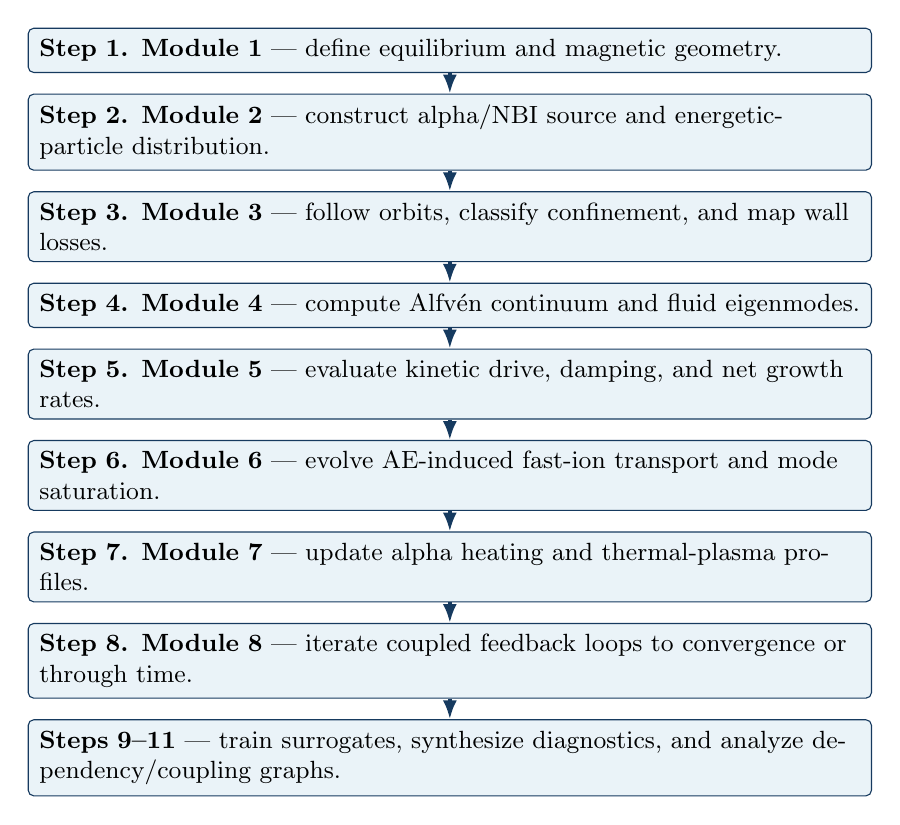
\begin{tikzpicture}[
node distance=2.6mm and 4mm,
box/.style={draw=accent, rounded corners=2pt, fill=accent2, minimum width=0.86\linewidth, text width=0.86\linewidth, align=left, inner sep=4pt, font=\small},
arrow/.style={-{Latex[length=2.4mm]}, very thick, draw=accent}
]
\node[box] (m1) {\textbf{Step 1. Module 1} --- define equilibrium and magnetic geometry.};
\node[box, below=of m1] (m2) {\textbf{Step 2. Module 2} --- construct alpha/NBI source and energetic-particle distribution.};
\node[box, below=of m2] (m3) {\textbf{Step 3. Module 3} --- follow orbits, classify confinement, and map wall losses.};
\node[box, below=of m3] (m4) {\textbf{Step 4. Module 4} --- compute Alfv\'en continuum and fluid eigenmodes.};
\node[box, below=of m4] (m5) {\textbf{Step 5. Module 5} --- evaluate kinetic drive, damping, and net growth rates.};
\node[box, below=of m5] (m6) {\textbf{Step 6. Module 6} --- evolve AE-induced fast-ion transport and mode saturation.};
\node[box, below=of m6] (m7) {\textbf{Step 7. Module 7} --- update alpha heating and thermal-plasma profiles.};
\node[box, below=of m7] (m8) {\textbf{Step 8. Module 8} --- iterate coupled feedback loops to convergence or through time.};
\node[box, below=of m8] (m9) {\textbf{Steps 9--11} --- train surrogates, synthesize diagnostics, and analyze dependency/coupling graphs.};
\draw[arrow] (m1) -- (m2);
\draw[arrow] (m2) -- (m3);
\draw[arrow] (m3) -- (m4);
\draw[arrow] (m4) -- (m5);
\draw[arrow] (m5) -- (m6);
\draw[arrow] (m6) -- (m7);
\draw[arrow] (m7) -- (m8);
\draw[arrow] (m8) -- (m9);
\end{tikzpicture}
\end{center}

\section{Coupling strategy}
The coupling sequence is not treated as an unconstrained machine-learning problem. Physical causality, conservation, and timescale separation define the admissible search space. Candidate numerical strategies include:
\begin{itemize}[leftmargin=1.6em]
\item one-way initialization followed by staggered Picard iteration;
\item block Gauss--Seidel exchange for tightly coupled feedback groups;
\item under-relaxation or Anderson acceleration;
\item waveform relaxation for modules with different natural time steps;
\item quasi-Newton coupling for the $f_f$--AE growth--transport loop;
\item conservative remapping between phase-space, radial-profile, and wall meshes;
\item learned closures only when a hard residual or conservation check remains available.
\end{itemize}
A generic coupling objective is
\begin{equation}
\mathcal J_{\mathrm{coupling}}=w_E\epsilon_E+w_N\epsilon_N+w_B\epsilon_{\nabla\cdot B}+w_R\lVert\mathbf R\rVert+w_I N_{\mathrm{iter}}+w_t t_{\mathrm{wall}}.
\end{equation}

\section{Core state and data interfaces}
\begin{longtable}{p{0.25\linewidth} p{0.29\linewidth} p{0.36\linewidth}}
\toprule
\textbf{State product} & \textbf{Produced by} & \textbf{Primary consumers}\\
\midrule
Equilibrium field and flux geometry & Module 1 & Modules 2--7\\
Energetic-particle source/distribution & Module 2 & Modules 3, 5, 6, and 7\\
Orbit frequencies and wall losses & Module 3 & Modules 5, 6, 7, and 10\\
Mode frequency and structure & Module 4 & Modules 5, 6, 9, and 10\\
Growth/damping rates and resonances & Module 5 & Modules 6, 8, 9, and 10\\
Transport coefficients and redistributed $f_f$ & Module 6 & Modules 2, 3, 7, and 8\\
Thermal-plasma profiles & Module 7 & Modules 1, 2, 4, 5, and 8\\
Coupled trajectories and residuals & Module 8 & Modules 9--11\\
Surrogate predictions and uncertainty & Module 9 & Module 8 and rapid-scan workflows\\
Synthetic diagnostic observations & Module 10 & Inverse-model and validation studies\\
Dependency graph and coupling recommendation & Module 11 & Module 8 solver-design studies\\
\bottomrule
\end{longtable}

\section{Parallel Python and MATLAB development}
The project maintains two independent implementations of the same physical architecture. The language trees shall share module numbering, governing equations, normalization conventions, configuration inputs, state-product names, verification cases, and output definitions. The MATLAB tree uses package directories beginning with \texttt{+}, which are the language-specific equivalent of Python package directories.

The implementations should not become line-by-line translations. Independent discretizations and language ecosystems provide a useful cross-check, but numerical agreement alone is not validation. Each implementation must separately satisfy dimensional checks, analytic limits, conservation diagnostics, convergence studies, and external reference comparisons. Shared data and configuration files remain at the repository root to prevent silent divergence of physical assumptions.

\section{Repository file map}
\begin{longtable}{p{0.31\linewidth} p{0.59\linewidth}}
\toprule
\textbf{Path} & \textbf{Role}\\
\midrule
\path{README.md} & Repository summary, current status, and entry point.\\
\path{project_plan.tex/.pdf} & Single living roadmap for architecture, coupling, interfaces, and implementation order.\\
\path{docs/shared/project_style.tex} & Shared LaTeX style inherited from the Radiation Effects project and renamed for this project.\\
\path{docs/physics_notes/} & Advanced module derivations and physics notes.\\
\path{docs/physics_notes/basics/} & One hundred stable prerequisite-note sources: thirty standalone textbook drafts, seventy scaffolds, a compiled status-aware index, and a machine-readable manifest.\\
\path{docs/implementation_notes/} & Module software contracts, algorithms, verification cases, and interface notes.\\
\path{python/src/kinetic_mhd_pinn/} & Python package arranged by physical module plus common state and coupling utilities.\\
\path{matlab/src/+kinetic_mhd_pinn/} & MATLAB package mirror with the same module contracts and language-appropriate classes/functions.\\
\path{python/cases/, matlab/cases/} & Reproducible benchmark and demonstration drivers in both languages.\\
\path{python/tests/, matlab/tests/} & Contract, verification, cross-language, and later regression tests.\\
\path{configs/} & Version-controlled run configurations.\\
\path{data/raw,processed,reference/} & Input, transformed, and benchmark/reference datasets.\\
\bottomrule
\end{longtable}

\section{Verification hierarchy}
Every implemented module should pass four levels of evidence:
\begin{enumerate}[leftmargin=1.6em]
\item \textbf{Dimensional and sign checks:} units, normalizations, conserved quantities, and direction conventions.
\item \textbf{Analytic limits:} uniform fields, no-drive limits, zero-gradient distributions, decoupled modes, and manufactured solutions.
\item \textbf{Cross-solver comparison:} independent Python and MATLAB implementations, independent discretizations, conventional solver versus PINN, or reduced model versus external reference data.
\item \textbf{Coupled diagnostics:} particle and energy budgets, mode-energy exchange, profile consistency, convergence, and sensitivity to exchange cadence.
\end{enumerate}

\section{Recommended coding order}
\begin{enumerate}[leftmargin=1.6em]
\item \textbf{Completed conventional stage:} implement Module 4 as a reduced two-harmonic TAE-like eigenvalue benchmark independently in Python and MATLAB, with frozen reference outputs and convergence tests.
\item Implement the Module 4 eigenvalue PINN and validate it against the conventional matrix solver.
\item Add Module 2 as a parameterized slowing-down energetic-particle distribution.
\item Implement a reduced Module 5 kinetic-drive closure and produce stability maps.
\item Add Module 6 one-dimensional quasilinear redistribution and mode-amplitude saturation.
\item Couple Module 7 profile/heating evolution and compare explicit, staggered, and accelerated coupling.
\item Introduce Module 1/3 stellarator geometry and guiding-center orbits after the reduced AE loop is verified.
\item Add Modules 9--11 only after credible conventional-solver datasets exist.
\end{enumerate}

\section{Milestone status and forward path}
\begin{longtable}{p{0.20\linewidth} p{0.38\linewidth} p{0.32\linewidth}}
\toprule
\textbf{Status} & \textbf{Milestone} & \textbf{Evidence or next acceptance criterion}\\
\midrule
Completed & Module 1 textbook physics note, version 1.0 & Comprehensive introductory-to-advanced treatment of stellarator equilibrium, flux surfaces, rotational transform, magnetic coordinates, three-dimensional Fourier geometry, equilibrium-solver concepts, output contracts, and verification; no three-dimensional solver is claimed.\\
Completed & Reduced two-harmonic Alfv\'en continuum/eigenmode benchmark & Python reference execution, matched MATLAB source, frozen CSV/JSON data products, continuum and eigenmode figures, scaling tests, decoupled-limit checks, and grid refinement.\\
Next & Module 4 eigenvalue PINN & Recover selected eigenfrequencies and eigenfunctions within prescribed tolerances while satisfying differential residuals, boundary conditions, normalization, and orthogonality.\\
Planned & Kinetic-drive stability map & Add a parameterized energetic-particle distribution, a reduced resonance/drive closure, net growth-rate scans, and uncertainty-aware surrogate comparison.\\
Planned & AE/fast-ion feedback loop & Add mode saturation, quasilinear redistribution, energy/particle diagnostics, and explicit versus staggered or accelerated coupling comparisons.\\
\bottomrule
\end{longtable}

\section{Current baseline boundary}
This baseline contains a completed Module 1 educational physics note and the first validated conventional numerical capability, but its executable scope remains intentionally reduced. It does not yet solve a three-dimensional stellarator equilibrium, guiding-center orbit populations, energetic-particle drive and damping, nonlinear fast-ion transport, alpha-heating feedback, synthetic diagnostics, or any PINN. The present Module 4 operator is a controlled two-harmonic radial benchmark for solver verification and future surrogate validation; it must not be represented as a predictive device-scale kinetic-MHD calculation. The next repository milestone is the Module 4 eigenvalue PINN, retained alongside---not in place of---the conventional matrix solver.

\end{document}
